\section{Dataset}
\label{sec:Dataset}

To train a machine learning model effectively and achieve accurate market price predictions, it is crucial to have access to latest high quality data. 
For this report, the used data is obtained from the dataset \textit{"USA Comprehensive Motorcycles Dataset 9k+"}\cite{kaggle_1}
and \textit{"Motorcycle Specifications Dataset"}\cite{kaggle_2}, available on \textbf{kaggle.com}. Both are licensed under \textit{CC0:Public Domain}.\\
The former dataset provides market prices, model, mileage and year of manufacture for the most popular brands \textit{BMW}, \textit{KTM}, \textit{Royal Enfield}, \textit{Suzuki}, \textit{Yamaha} and \textit{Ducati}
up to 2023, covering a significant portion of the motorcycle market. The second dataset provides further 
details for most motorcycle models like displacement, power or number of cylinders.

\subsection{Preprocessing}

An important initial task for machine learning projects is the preprocessing of the dataset. The complexity of this task varies strongly depending 
on the underlying quality of the data. As for the dataset used in this report, this step took longer than anticipated. As the data for all brands
were provided separately, one major task was to both merge all brand datasets into one and following that, merging the resulting dataset with the one containing further
details about the model specifications. An excerpt of the used datasets is shown in \autoref{fig:Bike_Tables_raw}. An enlarged view of the
datasets is shown in the \autoref{sec:Appendix}.
\begin{figure}
    \centering
    \begin{subfigure}[h]{0.325\textwidth}
        \centering
        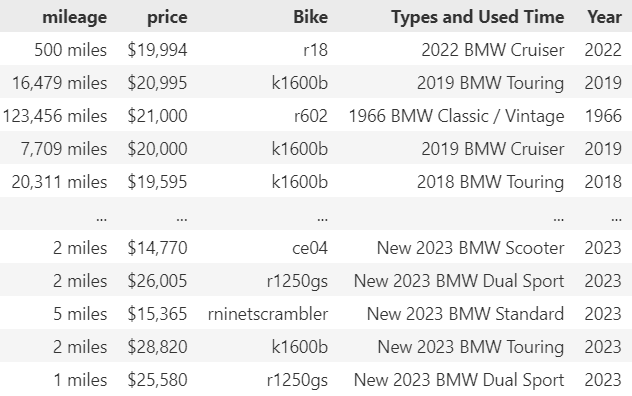
\includegraphics[width=\textwidth]{"content/pics/df_bmw_raw.png"}
    \end{subfigure}
    \hfill
    \begin{subfigure}[h]{0.66\textwidth}
        \centering
        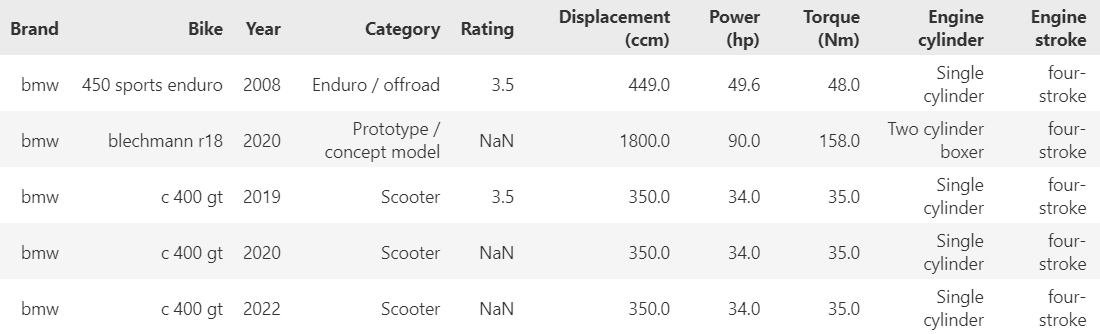
\includegraphics[width=\textwidth]{"content/pics/df_bikez_raw.png"}
    \end{subfigure}
    \caption{Excerpt of one of the brand datasets (BMW) containing price and selling specifications (left) and the dataset
    containing further model specifications (right).}
    \label{fig:Bike_Tables_raw}
\end{figure}
\\ Before merging all datasets, it is necessary to clean the columns properly. For this purpose, a descriptive column of the brand datasets
was discarded, due to its lack of consistently formatted data. Some entries of the removed column provided details about
the bike's condition or the limitation of the model. Additionally, the year of manufacture was extracted from the \textit{Types and Used Time}
column and all entries with no information on the price and mileage were dropped. The \textit{Bike} column of the price datasets
and the \textit{Bike} column of the specifications dataset were brought to the same formatting and style, such that a merge is possible.\\
The datasets are combined, based on the bike and the year of manufacture column. In cases with no matching
bike model for the exact year of manufacture in the specifications dataset, the entries are merged with another year of manufacture 
of that model. Some bike models of the specifications dataset are missing some column entries like \textit{Category} for specific years
of manufacture. These entries were filled with data from matching bike models from different years of manufacture.
At this stage, all entries for which the column \textit{Category} is empty are dropped.\\
\texttt{NaN} entries are filled with the mean value of the corresponding bike category. Additionally, the \textit{mileage} and  \textit{price} column data types are converted 
into integers the values and transformed into kilometres and euros instead of miles and dollars.\\
All brand subsets are concatenated to form one comprehensive dataset. A new condition column containing boolean values for 
Used (\texttt{True}) and New (\texttt{False}) is created based on the mileage. The \textit{Year} column is exchanged with the relative \textit{Age [a]} of the bike.
The final columns selected for further analysis are chosen as \textit{Mileage [km], Price [€], Bike, 
Brand, Category, Displacement [ccm], Power [hp], Torque [Nm], Condition} and \textit{Age [a]}. Data entries with a price larger than $\qty{50000} €$
are removed, since they are most likely limited editions.
\subsection{Exploratory Data Analysis}
\label{sec:Expl}
Before applying machine learning algorithms to the dataset and hoping for good results, it is important to first analyze 
the data distributions, correlations between attributes and explore useful data scaling methods.
As some of the columns contain categorical data (like \textit{Bike}), it is essential to convert them into numerical 
data for plotting purposes. For the \textit{Bike} and \textit{Category} column, a frequency mapping approach is chosen, meaning
that the categorical entries are replaced with their corresponding frequency in the dataset. This is a common approach for categorical columns
with a wide variety of entries. For the \textit{Brand} column, a dummy column is created. This means,
that for each unique value of the respective column, a new column with boolean values is created. \\
To gain a general understanding of the data distributions, a scatter matrix containing all columns (except the dummy columns) 
is presented in \autoref{fig:Scatterplot_All}.
\begin{figure}[h]
    \centering
        \makebox[\textwidth][h]{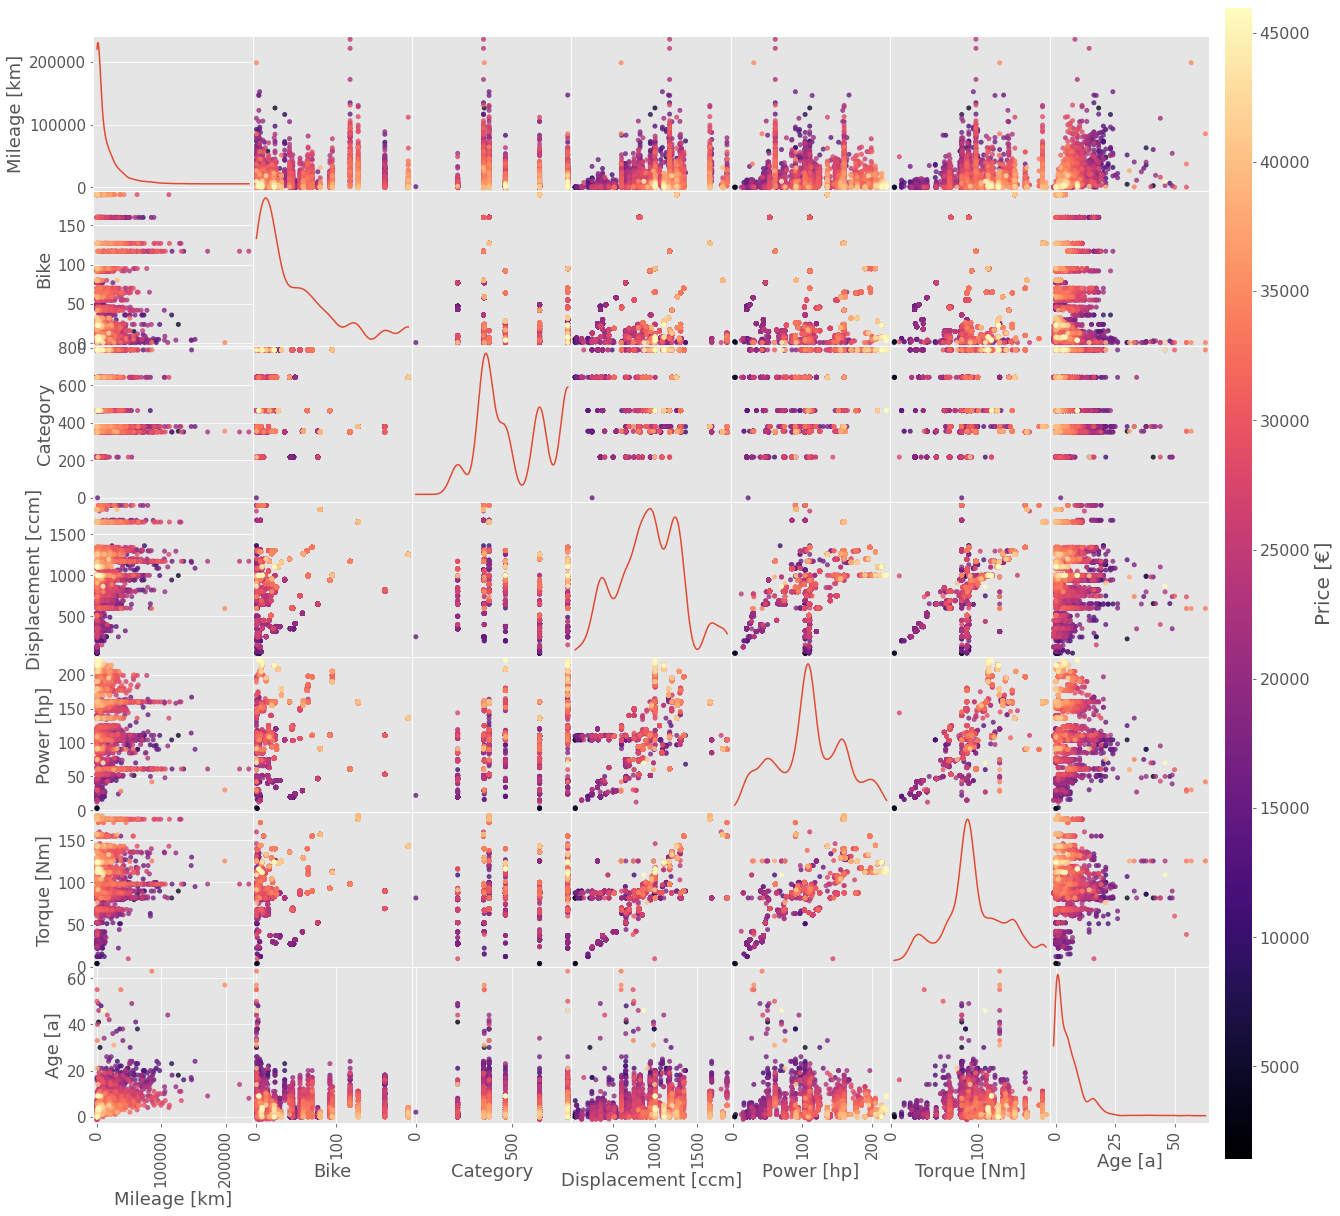
\includegraphics[width=0.9\textwidth]{"content/pics/Scatter_Matrix_All.png"}}
        \caption{Scatter matrix of all dataset attributes (except dummy columns) with their histograms presented on the diagonal.}
        \label{fig:Scatterplot_All}
\end{figure}
\\ It is evident that there is a significant amount of newer motorcycles with low age and mileage. The distribution of displacement,
power and torque is mostly normal, with significant peaks around the mean values, which is due to the filling of \texttt{NaN}
values with the mean. Several scatter plots show strong correlations, such as \textit{Power [hp]} and \textit{Torque [Nm]} (which
is very much expected due to their causal link). The \autoref{fig:Scatterplot_Price} shows clear dependencies
between the price and attributes, indicating their usefulness for regression problems.
\begin{figure}
    \centering
        \makebox[\textwidth][h]{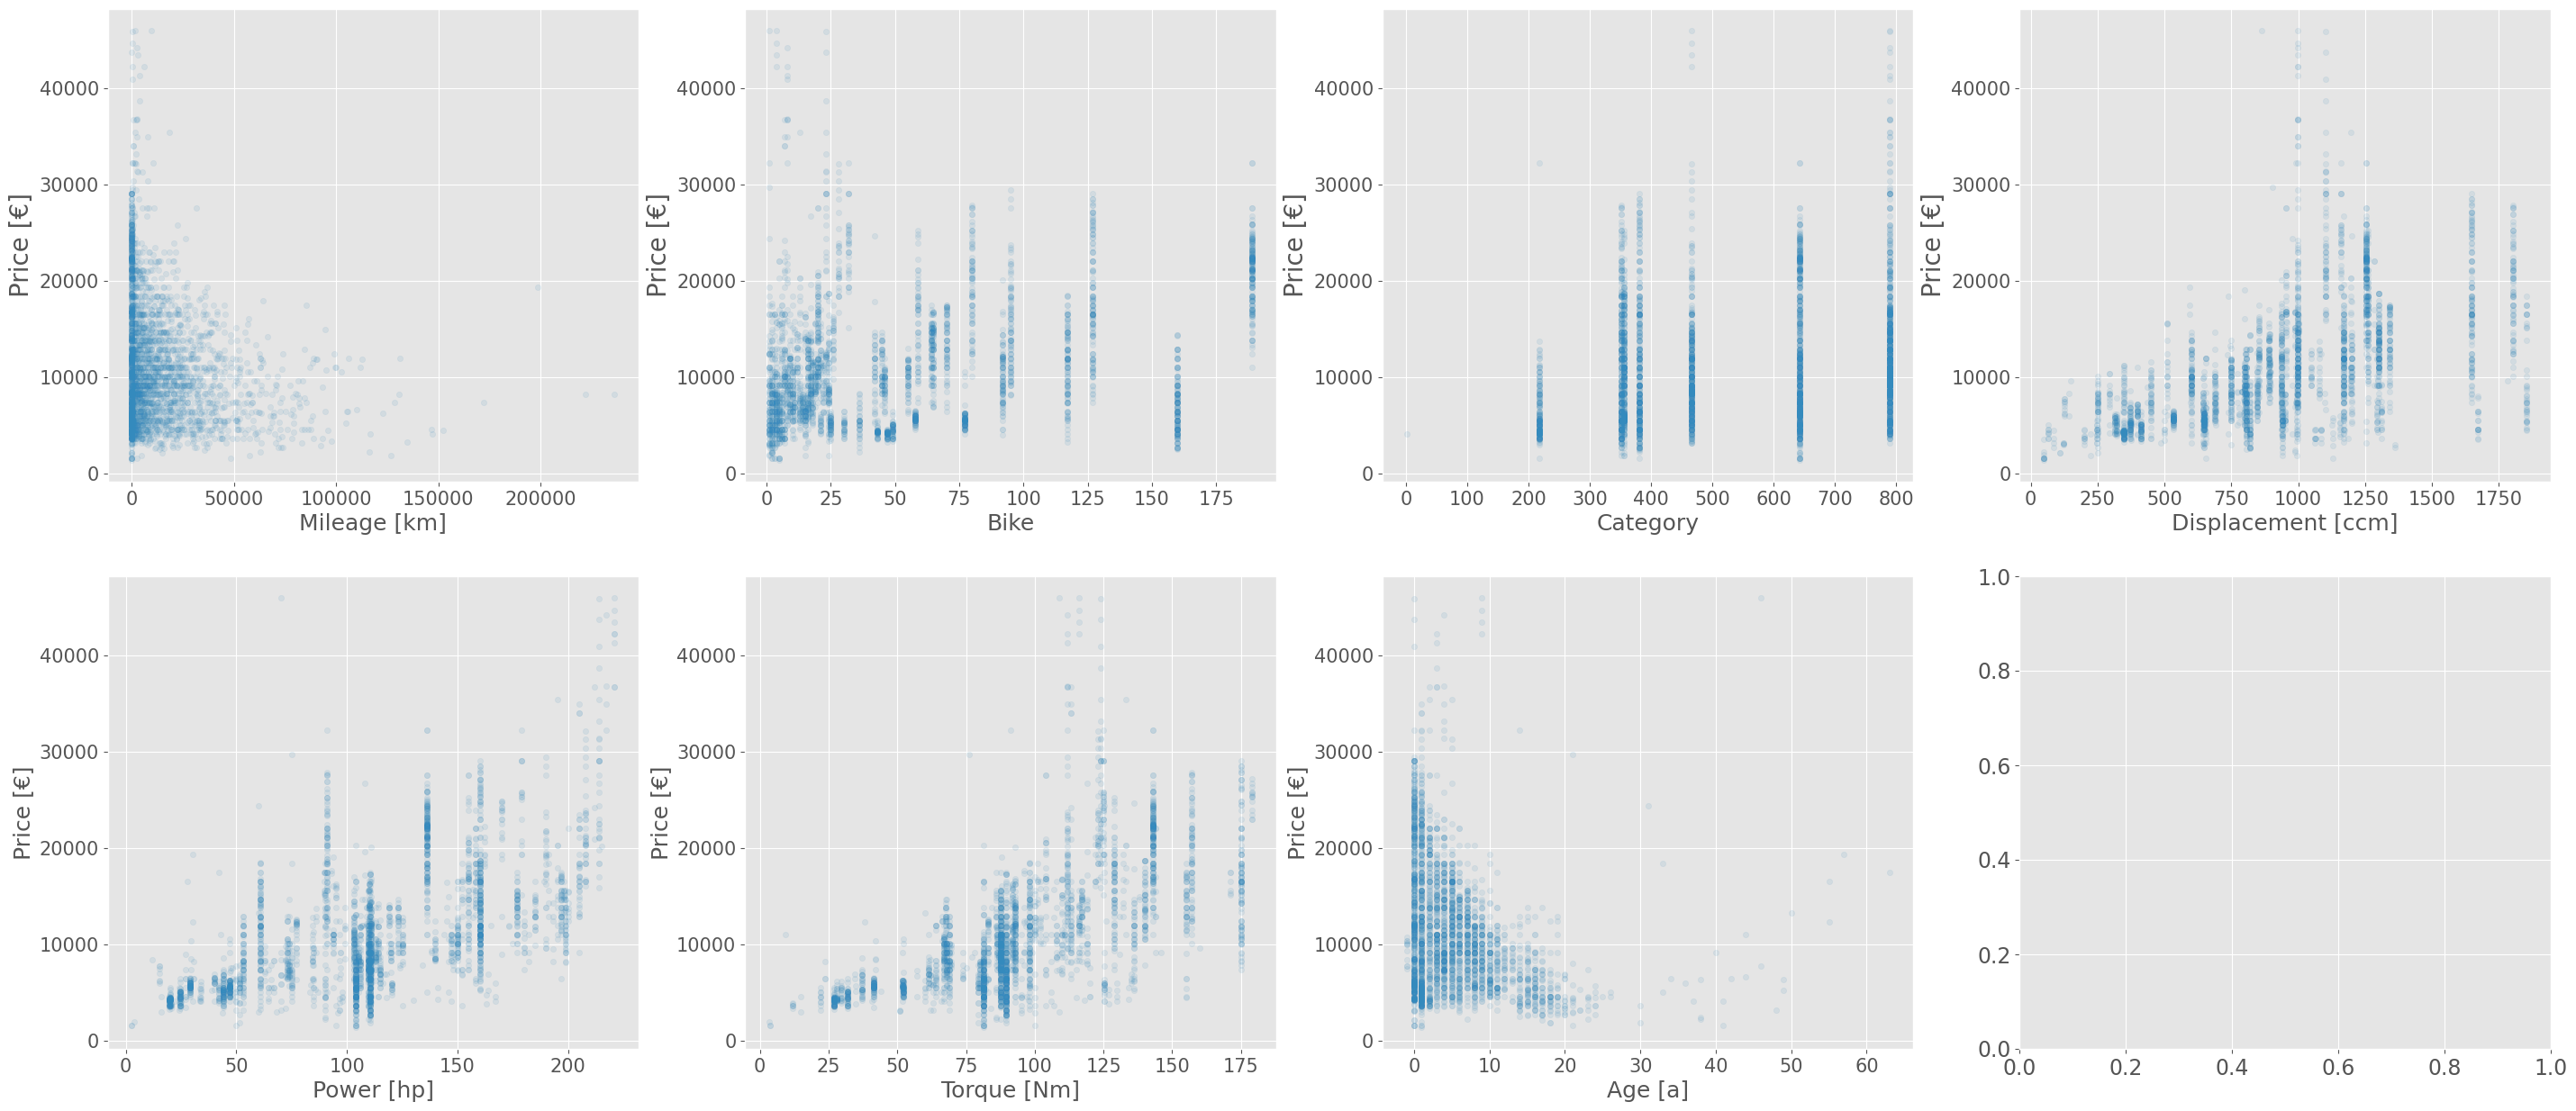
\includegraphics[width=1\textwidth]{"content/pics/Price_Attribute_Scatter.png"}}
        \caption{Scatter plots of the training attributes with the target value (\textit{Price [€]}).}
        \label{fig:Scatterplot_Price}
\end{figure}
\\When handling large datasets with a high amount of attributes and a very significant amount of data entries, long training times, 
overtraining and long waiting times for hyperparameter optimization is inevitable. Hence, it is crucial to take the correlations
among the used attributes into account. The correlation matrix for all attributes is shown in \autoref{fig:Corr_matrix}.
\begin{figure}[!]
    \centering
        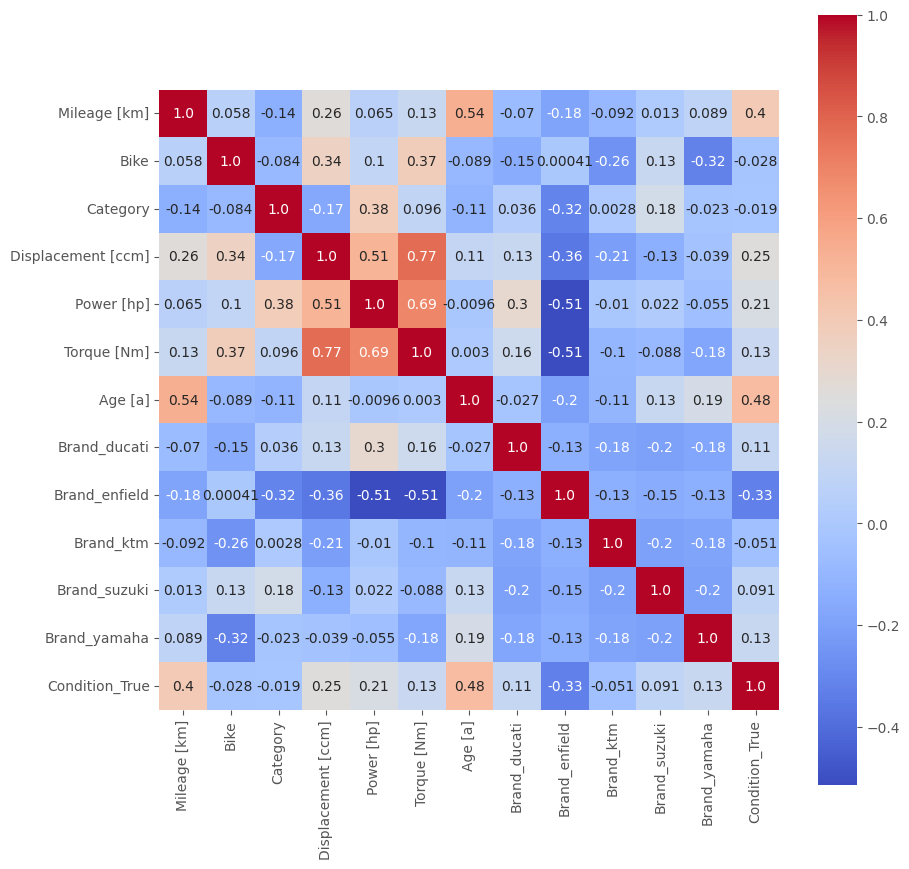
\includegraphics[width=0.7\textwidth]{"content/pics/correlation_matrix.png"}
        \caption{Correlation matrix of the used dataset attributes with encoded categorical columns.}
        \label{fig:Corr_matrix}
\end{figure}
\\The attributes such as torque, power and displacement show high correlation, which is expected given their mechanical nature.
Similarly, mileage and age, as well as the brand \textit{Royal Enfield} and the torque are highly correlated. However, at this stage,
no variables are discarded, due to the already limited number of attributes and the later performed feature selection.\\
Another effective method is to explore the behaviour of the data after applying different scaling transformations. 
The different scaling methods are observed for the \textit{Mileage} and \textit{Age} attributes, as they display the most continuous distribution and correlation with the price.
and nice correlations with the price. The scatter plots for these two attributes showcasing the \textit{"Standard"}, \textit{R"obust}, \textit{"Gaussian"},
\textit{"Min-Max"}, \textit{"Max-Abs"} and \textit{"Uniform"} scaling methods are shown in the \autoref{sec:Appendix}. The online documentation offers 
further insides on the transformations applied.
In the training of the individual regressor models, the standard, robust and normalised scaling are compared with no scaling.

